\documentclass{article}
\usepackage[utf8x]{inputenc}
\usepackage{polski}
\usepackage{pythonhighlight}

\usepackage{amssymb, amsmath, amsfonts, amsthm, cite, mathtools, enumerate, rotating, hyperref,soul, graphicx}
\newcommand \eq[1]{\begin{equation} \begin{split}  #1 \end{split} \end{equation}}

\makeatletter
\newcommand\tab[1][1cm]{\hspace*{#1}}
\def\@seccntformat#1{%
  \expandafter\ifx\csname c@#1\endcsname\c@section\else
  \csname the#1\endcsname\quad
  \fi}
\makeatother

\newtheorem{lemma}{Lemat}
\newtheorem{theorem}{Twierdzenie}

\title{AiSD L6}
\date{19.05.2021}
\author{Maurycy Borkowski}
\begin{document}
\maketitle
\section{zadanie 3.}
Chcemy sprowadzić problem z zadania do problemu stwierdzania izomomorfizmu pomiędzy dwoma ukorzenionymi drzewami.\\\\
\begin{lemma}Wierzchołek centralny $c$ leży na środku najdłuższej ścieżki.\end{lemma}
\begin{proof}
Załóżmy, niewprost że tak nie jest oznaczmy $c^\prime$ wierzchołek w środku najdłuższej ścieżki $u \leftrightarrow v$. Wtedy odległość $dist(c^\prime,u) = dist(c^\prime,v) \pm 1$ ale $\max \{dist(c,u), dist(c,v)\} > \max \{dist(c^\prime,u), dist(c^\prime,v)\}$ stąd $c$ nie jest wierzchołkiem centralnym. Sprzeczność.
\end{proof}
Okazuje się, że możemy ukorzenić drzewa w wierzchołkach centralnych.\\\\
Jeżeli istnieje izomomorfizm to wierzchołek centralny musi przechodzić na wierzchołek centralny. Najdłuższa ścieżka przechodzi na najdłuższą ścieżkę, a wierzchołek centralny leży w jej środku.\\\\
\subsection*{Szukanie centralnych}
Wierzchołek centralny musi(szą) leżeć na pewnej najdłuższej ścieżce (minimalizują one najdłuższą odległość od innych punktów). Stąd możemy po prostu iteracyjnie obrywać drzewo z liści, aż zostaną conajwyżej dwa wierzchołki.
\clearpage
\section{zadanie 4.}
Pokolorujmy wierzchołki w drzewie Algorytmu Hoare'a:
\begin{itemize}
  \item \textbf{Czerwony} korzeń i wierzchołki, które mają tablicę rozmiaru co najwyżej $\frac 3 4 x$ gdzie $x$ to rozmiar tablicy rodzica
  \item \textbf{Niebieski} pozostałe wierzchołki
\end{itemize}
Czerwone wierzchołki numerujemy od korzenia w dół $l$.\\\\
Rozmiar tablicy w każdym czerwonym wierzchołku jest ograniczony $\leq \left ( \frac{3}{4}\right)^l\cdot n$\\\\
Prawdopobieństwo posiadania niebieskiego syna ograniczamy przez $\frac 1 2$ musimy coś wybrać z pierwszej lub czwartej \textit{kwarty}. Stąd prawdopodobieństwo posiadania $k$ spójnych niebieskich potomków wynosi $2^{-k}$.\\Wartość oczekiwana niebieskiej lini potomstwa wynosi więc:
$$
\sum_{k=0}^{\infty} k \cdot 2^{-k} = 2
$$
Każdy wierzchołek wykonuje liniowo operacji na swojej tablicy ($\mathcal{O}(n)$).\\Zakładamy, że każdy $j$-ty czerwony wierzchołek ma dwóch niebieskich synów, ich tablice ograniczamy z góry przez tablice czerwonego przodka $\left ( \frac{3}{4}\right)^l\cdot n$. Stąd wykonujemy dla każdego zestawu (cz-n-n):
$$
(1+2)\cdot \left( \frac{3}{4}\right)^l\cdot \mathcal{O}(n)
$$
W takim razie możemy oszacować oczekiwaną złożoność algorytmu z góry przez:
$$
\sum_{l=0}^{\infty} (1+2)\cdot \left( \frac{3}{4}\right)^l\cdot \mathcal{O}(n) = \sum_{l=0}^{\infty} \left( \frac{3}{4}\right)^l\cdot \mathcal{O}(n) = \mathcal{O}(n) \cdot \sum_{l=0}^{\infty} \left( \frac{3}{4}\right)^l = \mathcal{O}(n) \cdot \frac{\frac{3}{4}}{1-\frac{3}{4}} = \mathcal{O}(n)
$$
\clearpage
\section{zadanie 5.}
\begin{lemma}
Długość najkrótszej ścieżki od korzenia do liścia wynosi co najwyżej $\log{(m+1)}$ gdzie $m$ to liczba wierzchołków w poddrzewie ukorzenionym w $x$.
\end{lemma}
\begin{proof}
Długość najkrótszej ścieżki od $x$ do liścia wynosi $h(x)$, stąd patrząc od góry od $x$ mamy \textbf{pełne} drzewo binarne o wsysokości $h(x)$. Zatem w tym drzewie mamy conajmniej $2^{h(x)}-1$ wierzchołków, jest to dolne ograniczenie na liczbę wierzchołków $2^{h(x)} - 1 \leq m$ stąd $h(x) \leq \log{(m+1)}$
\end{proof}
Obserwacja: najkrótsza ścieżka od korzenia do liścia jest w skrajnie prawej ścieżce.\\
Gdyby tak nie było to gdzieś musiałby być zaburzony niezmiennik.\\
\subsection*{Merge}
Sklejamy dwie skrajnie prawe ścieżki z $T_1,T_2$ (dwa posortowane ciągi) w jedną z $T$ (jeden posortowany ciąg). Jesteśmy w stanie to zrobić liniowo od długości tych ścieżek, które z lematu są długości conajwyżej logarytmicznej. Następnie naprawiamy $T$ dbając o niezmiennik. Jeżeli nie jest zachowany warunek zmieniamy synów miejscami. $\mathcal{O}(\log{|T_1|} + \log{|T_2|})$
\subsection*{Insert}
Tworzymy jedno elemntowe drzewo, łączymy je z drzewem.
\subsection*{Delete min/max}
Zastępujemy drzewo, złączeniem prawego i lewego syna korzenia.
\begin{python}
# min heap
def merge(t1,t2):
  if t1 is NULL:
    return t2
  if t2 is NULL:
    return t1
  
  if t1.key > t2.key:
    t1,t2 = t2,t1

  t1.right = merge(t1.right, t2)

  if t1.left is NULL:
    t1.left, t1.right = t1.right, t1.left
    t1.h = 1
    return t1

  if t1.right.h > t1.left.h:
    t1.left, t1.right = t1.right, t1.left
  t1.h = t1.right.h + 1
  return t1
\end{python}
\clearpage
\section{zadanie 8.}
Drzewo AVL, ale trzymamy dodatkowe trzy informacje w wierzchołkach:
\begin{itemize}
  \item $mindiff$ - wartość $mindiff$ w danym poddrzewie
  \item $min$ - minimum w poddrzewie
  \item $max$ - maximum w poddrzewie
\end{itemize}
$mindiff$ wyznaczamy (uważając na nulle):
\begin{align*}
mindiff = \min \{ 
  mindiff \text{  lewego syna}\\
  mindiff \text{  prawego syna}\\
  v - lewy.max\\
  prawy.min - v\}
\end{align*}
\textbf{Mindiff} Zwracamy wartość $mindiff$ korzenia.\\
\textbf{Insert/Delete} Aktualizujemy tylko wierzchołki na ścieżce od usuwane/dodanego wierzchołka do korzenia. Uaktualniamy $min, max, mindiff$.\\
\textbf{Rotacja}\\
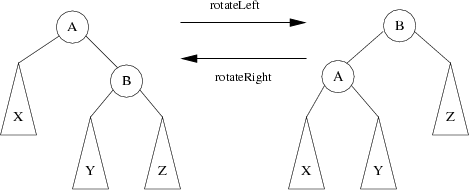
\includegraphics[scale=0.7]{rotacje}\\
\textbf{rotacja lewa}\\
Najpierw updatujemy $min/max$ a potem na podstawie tego $mindiff$:\\\\
$A.max$ zmieniamy na $Y.max$\\
$B.min$ zmieniamy na $A.min$\\\\
\textbf{rotacja prawa} analogicznie\\
\clearpage
\section{zadanie 9.}
\textbf{Obserwacja}\\
Zauważmy, że nie musimy trzymać wartości o wyważeniu, w wierzchołkach, które mają conajwyżej $1$ syna. W liściach, lub z jednym synem mamy odpowiednio wyważenie, albo przeciążenie w stronę jedynaka.\\\\
W szczególności \textit{ostatnie piętro} samych liści nie potrzebuje trzymać tej informacji. Możemy więc zepchnąć te wartości o jeden poziom w dół. Każdy wierzchołek trzyma po jednym bicie w każdym swoim z dwóch synów, w ten sposób możemy trzymać informacje z $4$ stanami (potrzebujemy $3$) w każdym dwuliściowym wierzchołku (inne nie intersują nas z obserwacji).
\end{document}